% Options for packages loaded elsewhere
% Options for packages loaded elsewhere
\PassOptionsToPackage{unicode}{hyperref}
\PassOptionsToPackage{hyphens}{url}
\PassOptionsToPackage{dvipsnames,svgnames,x11names}{xcolor}
%
\documentclass[
  authoryear,
  preprint]{elsarticle}
\usepackage{xcolor}
\usepackage{amsmath,amssymb}
\setcounter{secnumdepth}{5}
\usepackage{iftex}
\ifPDFTeX
  \usepackage[T1]{fontenc}
  \usepackage[utf8]{inputenc}
  \usepackage{textcomp} % provide euro and other symbols
\else % if luatex or xetex
  \usepackage{unicode-math} % this also loads fontspec
  \defaultfontfeatures{Scale=MatchLowercase}
  \defaultfontfeatures[\rmfamily]{Ligatures=TeX,Scale=1}
\fi
\usepackage{lmodern}
\ifPDFTeX\else
  % xetex/luatex font selection
\fi
% Use upquote if available, for straight quotes in verbatim environments
\IfFileExists{upquote.sty}{\usepackage{upquote}}{}
\IfFileExists{microtype.sty}{% use microtype if available
  \usepackage[]{microtype}
  \UseMicrotypeSet[protrusion]{basicmath} % disable protrusion for tt fonts
}{}
\makeatletter
\@ifundefined{KOMAClassName}{% if non-KOMA class
  \IfFileExists{parskip.sty}{%
    \usepackage{parskip}
  }{% else
    \setlength{\parindent}{0pt}
    \setlength{\parskip}{6pt plus 2pt minus 1pt}}
}{% if KOMA class
  \KOMAoptions{parskip=half}}
\makeatother
% Make \paragraph and \subparagraph free-standing
\makeatletter
\ifx\paragraph\undefined\else
  \let\oldparagraph\paragraph
  \renewcommand{\paragraph}{
    \@ifstar
      \xxxParagraphStar
      \xxxParagraphNoStar
  }
  \newcommand{\xxxParagraphStar}[1]{\oldparagraph*{#1}\mbox{}}
  \newcommand{\xxxParagraphNoStar}[1]{\oldparagraph{#1}\mbox{}}
\fi
\ifx\subparagraph\undefined\else
  \let\oldsubparagraph\subparagraph
  \renewcommand{\subparagraph}{
    \@ifstar
      \xxxSubParagraphStar
      \xxxSubParagraphNoStar
  }
  \newcommand{\xxxSubParagraphStar}[1]{\oldsubparagraph*{#1}\mbox{}}
  \newcommand{\xxxSubParagraphNoStar}[1]{\oldsubparagraph{#1}\mbox{}}
\fi
\makeatother

\usepackage{color}
\usepackage{fancyvrb}
\newcommand{\VerbBar}{|}
\newcommand{\VERB}{\Verb[commandchars=\\\{\}]}
\DefineVerbatimEnvironment{Highlighting}{Verbatim}{commandchars=\\\{\}}
% Add ',fontsize=\small' for more characters per line
\usepackage{framed}
\definecolor{shadecolor}{RGB}{241,243,245}
\newenvironment{Shaded}{\begin{snugshade}}{\end{snugshade}}
\newcommand{\AlertTok}[1]{\textcolor[rgb]{0.68,0.00,0.00}{#1}}
\newcommand{\AnnotationTok}[1]{\textcolor[rgb]{0.37,0.37,0.37}{#1}}
\newcommand{\AttributeTok}[1]{\textcolor[rgb]{0.40,0.45,0.13}{#1}}
\newcommand{\BaseNTok}[1]{\textcolor[rgb]{0.68,0.00,0.00}{#1}}
\newcommand{\BuiltInTok}[1]{\textcolor[rgb]{0.00,0.23,0.31}{#1}}
\newcommand{\CharTok}[1]{\textcolor[rgb]{0.13,0.47,0.30}{#1}}
\newcommand{\CommentTok}[1]{\textcolor[rgb]{0.37,0.37,0.37}{#1}}
\newcommand{\CommentVarTok}[1]{\textcolor[rgb]{0.37,0.37,0.37}{\textit{#1}}}
\newcommand{\ConstantTok}[1]{\textcolor[rgb]{0.56,0.35,0.01}{#1}}
\newcommand{\ControlFlowTok}[1]{\textcolor[rgb]{0.00,0.23,0.31}{\textbf{#1}}}
\newcommand{\DataTypeTok}[1]{\textcolor[rgb]{0.68,0.00,0.00}{#1}}
\newcommand{\DecValTok}[1]{\textcolor[rgb]{0.68,0.00,0.00}{#1}}
\newcommand{\DocumentationTok}[1]{\textcolor[rgb]{0.37,0.37,0.37}{\textit{#1}}}
\newcommand{\ErrorTok}[1]{\textcolor[rgb]{0.68,0.00,0.00}{#1}}
\newcommand{\ExtensionTok}[1]{\textcolor[rgb]{0.00,0.23,0.31}{#1}}
\newcommand{\FloatTok}[1]{\textcolor[rgb]{0.68,0.00,0.00}{#1}}
\newcommand{\FunctionTok}[1]{\textcolor[rgb]{0.28,0.35,0.67}{#1}}
\newcommand{\ImportTok}[1]{\textcolor[rgb]{0.00,0.46,0.62}{#1}}
\newcommand{\InformationTok}[1]{\textcolor[rgb]{0.37,0.37,0.37}{#1}}
\newcommand{\KeywordTok}[1]{\textcolor[rgb]{0.00,0.23,0.31}{\textbf{#1}}}
\newcommand{\NormalTok}[1]{\textcolor[rgb]{0.00,0.23,0.31}{#1}}
\newcommand{\OperatorTok}[1]{\textcolor[rgb]{0.37,0.37,0.37}{#1}}
\newcommand{\OtherTok}[1]{\textcolor[rgb]{0.00,0.23,0.31}{#1}}
\newcommand{\PreprocessorTok}[1]{\textcolor[rgb]{0.68,0.00,0.00}{#1}}
\newcommand{\RegionMarkerTok}[1]{\textcolor[rgb]{0.00,0.23,0.31}{#1}}
\newcommand{\SpecialCharTok}[1]{\textcolor[rgb]{0.37,0.37,0.37}{#1}}
\newcommand{\SpecialStringTok}[1]{\textcolor[rgb]{0.13,0.47,0.30}{#1}}
\newcommand{\StringTok}[1]{\textcolor[rgb]{0.13,0.47,0.30}{#1}}
\newcommand{\VariableTok}[1]{\textcolor[rgb]{0.07,0.07,0.07}{#1}}
\newcommand{\VerbatimStringTok}[1]{\textcolor[rgb]{0.13,0.47,0.30}{#1}}
\newcommand{\WarningTok}[1]{\textcolor[rgb]{0.37,0.37,0.37}{\textit{#1}}}

\usepackage{longtable,booktabs,array}
\usepackage{calc} % for calculating minipage widths
% Correct order of tables after \paragraph or \subparagraph
\usepackage{etoolbox}
\makeatletter
\patchcmd\longtable{\par}{\if@noskipsec\mbox{}\fi\par}{}{}
\makeatother
% Allow footnotes in longtable head/foot
\IfFileExists{footnotehyper.sty}{\usepackage{footnotehyper}}{\usepackage{footnote}}
\makesavenoteenv{longtable}
\usepackage{graphicx}
\makeatletter
\newsavebox\pandoc@box
\newcommand*\pandocbounded[1]{% scales image to fit in text height/width
  \sbox\pandoc@box{#1}%
  \Gscale@div\@tempa{\textheight}{\dimexpr\ht\pandoc@box+\dp\pandoc@box\relax}%
  \Gscale@div\@tempb{\linewidth}{\wd\pandoc@box}%
  \ifdim\@tempb\p@<\@tempa\p@\let\@tempa\@tempb\fi% select the smaller of both
  \ifdim\@tempa\p@<\p@\scalebox{\@tempa}{\usebox\pandoc@box}%
  \else\usebox{\pandoc@box}%
  \fi%
}
% Set default figure placement to htbp
\def\fps@figure{htbp}
\makeatother





\setlength{\emergencystretch}{3em} % prevent overfull lines

\providecommand{\tightlist}{%
  \setlength{\itemsep}{0pt}\setlength{\parskip}{0pt}}



 
\usepackage[]{natbib}
\bibliographystyle{elsarticle-harv}


\usepackage{booktabs}
\usepackage{caption}
\usepackage{longtable}
\usepackage{colortbl}
\usepackage{array}
\usepackage{anyfontsize}
\usepackage{multirow}
\makeatletter
\@ifpackageloaded{tcolorbox}{}{\usepackage[skins,breakable]{tcolorbox}}
\@ifpackageloaded{fontawesome5}{}{\usepackage{fontawesome5}}
\definecolor{quarto-callout-color}{HTML}{909090}
\definecolor{quarto-callout-note-color}{HTML}{0758E5}
\definecolor{quarto-callout-important-color}{HTML}{CC1914}
\definecolor{quarto-callout-warning-color}{HTML}{EB9113}
\definecolor{quarto-callout-tip-color}{HTML}{00A047}
\definecolor{quarto-callout-caution-color}{HTML}{FC5300}
\definecolor{quarto-callout-color-frame}{HTML}{acacac}
\definecolor{quarto-callout-note-color-frame}{HTML}{4582ec}
\definecolor{quarto-callout-important-color-frame}{HTML}{d9534f}
\definecolor{quarto-callout-warning-color-frame}{HTML}{f0ad4e}
\definecolor{quarto-callout-tip-color-frame}{HTML}{02b875}
\definecolor{quarto-callout-caution-color-frame}{HTML}{fd7e14}
\makeatother
\makeatletter
\@ifpackageloaded{caption}{}{\usepackage{caption}}
\AtBeginDocument{%
\ifdefined\contentsname
  \renewcommand*\contentsname{Table of contents}
\else
  \newcommand\contentsname{Table of contents}
\fi
\ifdefined\listfigurename
  \renewcommand*\listfigurename{List of Figures}
\else
  \newcommand\listfigurename{List of Figures}
\fi
\ifdefined\listtablename
  \renewcommand*\listtablename{List of Tables}
\else
  \newcommand\listtablename{List of Tables}
\fi
\ifdefined\figurename
  \renewcommand*\figurename{Figure}
\else
  \newcommand\figurename{Figure}
\fi
\ifdefined\tablename
  \renewcommand*\tablename{Table}
\else
  \newcommand\tablename{Table}
\fi
}
\@ifpackageloaded{float}{}{\usepackage{float}}
\floatstyle{ruled}
\@ifundefined{c@chapter}{\newfloat{codelisting}{h}{lop}}{\newfloat{codelisting}{h}{lop}[chapter]}
\floatname{codelisting}{Listing}
\newcommand*\listoflistings{\listof{codelisting}{List of Listings}}
\makeatother
\makeatletter
\makeatother
\makeatletter
\@ifpackageloaded{caption}{}{\usepackage{caption}}
\@ifpackageloaded{subcaption}{}{\usepackage{subcaption}}
\makeatother
\journal{Journal Name}
\usepackage{bookmark}
\IfFileExists{xurl.sty}{\usepackage{xurl}}{} % add URL line breaks if available
\urlstyle{same}
\hypersetup{
  pdftitle={Responsive Robotics to Increase Trust in Autonomous Human--Robot Interaction},
  pdfauthor={M.C. Lau; Shauna Heron},
  pdfkeywords={human-robot interaction, HRI, socially assistive
robotics, cobots, autonomous robot systems, spoken language
interaction, trust in automation, trust in human-robot
interaction, affect-adaptive systems},
  colorlinks=true,
  linkcolor={blue},
  filecolor={Maroon},
  citecolor={Blue},
  urlcolor={Blue},
  pdfcreator={LaTeX via pandoc}}


\setlength{\parindent}{6pt}
\begin{document}

\begin{frontmatter}
\title{Responsive Robotics to Increase Trust in Autonomous Human--Robot
Interaction \\\large{An In-Person Pilot Study} }
\author[1]{M.C. Lau%
\corref{cor1}%
\fnref{fn1}}
 \ead{mclau@laurentian.ca} 
\author[1]{Shauna Heron%
%
\fnref{fn2}}
 \ead{sheron@laurentian.ca} 

\affiliation[1]{organization={Laurentian University, Bharti School of
Engineering},,postcodesep={}}
\affiliation[2]{organization={Laurentian University, School of Social
Sciences},,postcodesep={}}

\cortext[cor1]{Corresponding author}
\fntext[fn1]{This is the first author footnote.}
\fntext[fn2]{Another author footnote, this is a very long footnote and
it should be a really long footnote. But this footnote is not yet
sufficiently long enough to make two lines of footnote text.}
        
\begin{abstract}
This study implements a multi-stage collaborative task system where
participants collaborate with the Misty-II social robot to solve a
who-dunnit type task. The system utilizes an autonomous,
mixed-initiative dialogue architecture with affect-responsive
capabilities.
\end{abstract}





\begin{keyword}
    human-robot interaction \sep HRI \sep socially assistive
robotics \sep cobots \sep autonomous robot systems \sep spoken language
interaction \sep trust in automation \sep trust in human-robot
interaction \sep 
    affect-adaptive systems
\end{keyword}
\end{frontmatter}
    

\subsection{Project Description}\label{project-description}

As many industries move toward greater automation (e.g., mining,
manufacturing), robotic assistants are becoming increasingly common in
operational workflows from manufacturing to mining
\citep{fu2021, racette2024}. These systems can help reduce human
exposure to hazards, but trust remains a critical barrier to adoption
\citep{campagna2025, emaminejad2022}. Low trust can lead to rejection of
automation, while excessive trust (automation bias) risks overreliance
\citep{devisser2020}. While most industrial robots rely on fixed,
rule-based behaviour, there is growing interest in AI-enhanced systems
that support more adaptive and socially intelligent interactions.

Research shows that emotional responsiveness in robots---expressed
through tone, facial expression, or supportive dialogue---can improve
perceptions of trustworthiness and social intelligence
\citep{shayganfar2019, fartook2025}. Moreover, a robot's ability to
detect early signs of stress, fatigue, or cognitive overload may have
practical value in high-risk environments such as underground mines,
where attentional lapses can pose serious safety risks
\citep{racette2024, murphy2009}. Responsive adaptation in this context
could enhance both trust and real-time situational awareness
\citep{fu2021, murphy2009, racette2024}.

This project aims to develop and evaluate a multi-sensor
Emotion-Adaptive AI System (EAI) for the Misty II robot \citep{mistya}.
The EAI will use AI-driven affect-inference models including facial
emotion recognition models, vocal tone analysis, combined with a
generative language model to coordinate task interaction monitoring to
estimate user affective states such as frustration, confusion, or
disengagement. These inferences will guide Misty's real-time responses,
including encouragement, clarification prompts, or praise. We will
compare this adaptive mode against a neutral, rule-based version of
Misty to assess effects on user trust, collaboration, and task
performance. We will also explore how individual cognitive traits may
moderate these interactions \citep{nicolas2021}.

\section{Pilot Study}\label{pilot-study}

Human--robot collaboration (HRC) has become a central topic across
engineering, computer science, and the social sciences as robots
increasingly move from controlled laboratory settings into everyday
collaborative roles. In many emerging applications, collaboration
depends not only on physical coordination but also on shared
problem-solving through dialogue, where AI-driven robots must reason,
communicate, and adapt in real time. Understanding how humans perceive
and respond to such systems is therefore critical for designing robots
that can function as effective collaborators rather than passive tools.

A key factor shaping successful collaboration in human--robot
interaction (HRI) is trust \citep{waytz2014, emaminejad2022}. Trust
influences whether users are willing to adopt robotic systems, accept
their guidance, and remain engaged during joint tasks, particularly in
situations characterized by uncertainty or incomplete information
\citep{waytz2014, emaminejad2022}. Prior work has shown that trust
affects both subjective perceptions such as perceived reliability or
intent, and objective outcomes including task performance, compliance,
and cooperation. As a result, a substantial body of research has focused
on measuring trust in HRI, leading to the development of standardized
instruments for assessing users' evaluations of robot behaviour across
industrial, medical, and social contexts.

Despite this progress, much of the existing literature on trust in HRI
is based on interactions conducted under highly controlled or simulated
conditions. In many studies, robot behaviour is scripted, partially
simulated, or mediated through Wizard-of-Oz paradigms, where a human
operator covertly controls aspects of the robot's behaviour. While these
approaches are valuable for isolating specific design factors and
testing early hypotheses, they also mask many of the failures and
inconsistencies that characterize autonomous systems in real-world use.
Speech recognition errors, delayed or inappropriate responses,
misinterpretations of user intent, and limitations of affect sensing are
not peripheral issues but central features of deployed autonomous
robots. These imperfections are likely to play a decisive role in
shaping trust, yet they remain underexplored in empirical HRI research.

Introduce the concept of responsiveness in robot/AI systems as a
moderator of trust. Prior work has suggested that robots that can adapt
their behaviour based on user affect and contextual cues may foster
greater trust and engagement. However, most studies examining
responsiveness have relied on simulated or semi-autonomous systems,
leaving open questions about how these effects manifest in fully
autonomous, in-person interactions. While most industrial robots rely on
fixed, rule-based behaviour, there is growing interest in AI-enhanced
systems that support more adaptive and socially intelligent interactions
\citep{fu2021, murphy2009, racette2024}.

The present pilot study addresses this gap by examining trust and
collaboration in an in-person interaction with two versions of a fully
autonomous social robot operating within predefined behavioural
constraints. Using a between-subjects design, participants collaborated
with either a responsive or neutral robot during an immersive,
dialogue-driven puzzle game in which the robot acted as a diegetic game
guide and partner. The task required shared problem-solving through
conversation, with participants seeking hints, advice, and support from
the robot while navigating a game environment displayed on a computer
screen. Crucially, all interaction management---including speech-based
dialogue, task progression, and affect-responsive behaviour was handled
autonomously by the robot without human intervention.

In the experimental condition, the robot was designed to be proactive
and responsive, adapting its behaviour based on participant affect--as
estimated from outputs of an affect detection model--as well as
conversational cues. In the other condition, the robot provided
assistance only when explicitly requested, offering a more reactive
interaction style. This manipulation allowed us to examine how
differences in autonomy and responsiveness to human states influence
trust perceptions and collaborative performance under otherwise
identical task demands.

To support this interaction, we developed an autonomous spoken-language
system integrated with automatic speech recognition (ASR) and affect
detection on the Misty-II robot platform. The system we developed
enables the robot to recognize speech, manage dialogue state, maintain
conversational context, and generate coordinated verbal responses
alongside LED facial expressions and head and arm movements. Rather than
optimizing for flawless performance, the system was designed to reflect
realistic capabilities and limitations of contemporary social robots.

By combining post-interaction trust measures with behavioural and
task-level outcomes, this study aims to contribute empirical evidence on
how trust is shaped in fully autonomous HRI scenarios. The focus is not
on demonstrating idealized interaction under perfect conditions, but on
examining trust as it emerges through realistic human--robot
collaboration, where uncertainty, interactional breakdowns, and adaptive
behaviour are unavoidable. In doing so, this work seeks to inform the
design and evaluation of affect-responsive autonomous robots intended
for real-world collaborative settings.

This project aimed to develop and evaluate a multi-sensor
Emotion-Adaptive AI System (EAI) for the Misty II robot \citep{mistya}.
The EAI leveraged pretrained LLMs for syntaxical affect inference and
task interaction monitoring to estimate user affective states such as
frustration, engagement, or anxiousness. These inferences guided Misty's
real-time responses, including encouragement, clarification prompts, and
praise. We compared an adaptive version of Misty against a neutral,
rule-based version of Misty to assess effects on user trust,
collaboration, and perceived intelligence. We also explored how
individual differences in Need for Cognition could moderate these
interactions \citep{nicolas2021}.

{[}also mention the pre-session questionnaire with NARS and NFC to
capture baseline attitudes and individual differences that may moderate
trust responses{]} {[}also mention that this is a pilot study to inform
a larger planned study with more participants and refined methods based
on lessons learned here and touch on some of the lessons we learned
(i.e., language issues, ASR issues, interaction design issues, etc.){]}

\subsection{Related work}\label{related-work}

\subsubsection{Spoken language interaction in
HRI}\label{spoken-language-interaction-in-hri}

Discuss prior work on spoken language interaction in HRI, including the
challenges of ASR, dialogue management, and affect detection in
real-world settings. Summarize key findings from studies that have
examined how spoken language capabilities influence user perceptions of
robots, particularly in collaborative tasks. Highlight any gaps in the
literature regarding fully autonomous systems operating in-person
without human intervention.

While most industrial robots rely on fixed, rule-based behaviour, there
is growing interest in AI-enhanced systems that support more adaptive
and socially intelligent interactions
\citep{fu2021, murphy2009, racette2024}. Discuss the technical
challenges of implementing spoken language interaction on mobile robot
platforms, including issues related to speech recognition accuracy,
latency, and contextual understanding. Explain how these challenges
impact user perceptions and trust in HRI.

\subsubsection{Trust in HRI research}\label{trust-in-hri-research}

Research shows that responsiveness to human-affect in robots---expressed
through tone, movement, facial expression, or supportive dialogue---can
improve perceptions of trustworthiness and social intelligence
\citep{shayganfar2019, fartook2025}. These anthropomorphic cues may
serve as transparency signals, helping users infer robotic intent and
fostering cooperation \citep{birnbaum2016}.

A robot's ability to detect and respond to early signs of stress,
fatigue, confusion or cognitive overload could have practical value in
high-risk environments like medical settings or underground mines where
attentional lapses pose serious safety risks. Affecctive adaptation in
these contexts could enhance both trust as well as real-time
responsiveness and situational awareness
\citep{fu2021, murphy2009, racette2024}.

Introduce the two scales here we used to measure trust in HRI: adapted
14-item Trust Perception Scale-HRI \citep{bartneck2009} and the Trust in
Industrial Human--Robot Collaboration scale \citep{charalambous}.
Discuss prior work that has used these scales and their relevance to our
study. The differences between these two scales in terms of what aspects
of trust they measure (e.g., affective vs.~cognitive trust, reliability
vs.~collaboration). In addition, discuss how these scales have been
validated in prior research and their psychometric properties.

Also talk about using the Negative Attitudes Toward Robots Scale (NARS)
\citep{nomura2006} and the Need for Cognition Scale (NFC-s)
\citep[\citet{cacioppo1996}]{cacioppo1984} as baseline measures to
account for individual differences in attitudes toward robots and
cognitive engagement that may influence trust perceptions.

Explain why we chose to use both scales in our study to capture a
comprehensive picture of trust in HRI. The reasons for selecting these
scales should be linked to our research questions and hypotheses about
how robot responsiveness and affective adaptation might influence
different dimensions of trust.

\subsubsection{Responsiveness and affective adaptation in
HRI}\label{responsiveness-and-affective-adaptation-in-hri}

Discuss prior research on the role of robot responsiveness and affective
adaptation in shaping trust and engagement in HRI. Summarize key
findings from studies that have examined how robots that can perceive
and respond to human affective states influence user perceptions and
behaviours. Highlight any gaps in the literature, particularly regarding
fully autonomous, in-person interactions, which our study aims to
address.

Discuss theoretical frameworks that explain why responsiveness and
affective adaptation might enhance trust, such as social presence theory
or the CASA paradigm. Explain how these frameworks inform our hypotheses
about the expected effects of robot interaction policy on trust and
collaboration.

Discuss the reason for conducting the study in a fully autonomous,
in-person setting rather than using Wizard-of-Oz or simulated paradigms.
Emphasize the importance of examining trust in realistic conditions
where interaction imperfections are present.

\subsubsection{Why a pilot study?}\label{why-a-pilot-study}

Why did we run a pilot study? what future work will this inform? Focus
on testing feasibility of the autonomous system, interaction design, and
measurement approach.

Our initial objectives: 1. Develop and implement an autonomous
Emotion-Adaptive AI System (EAI) using Misty's onboard sensor data and
AI on an edge device. 2. Evaluate the impact of EAI on trust, perceived
social intelligence, and task collaboration in two types of human-robot
tasks. 3. Assess whether individual differences in human cognitive style
(i.e., Need for Cognition) influences responses to adaptive robotic
behaviour and trust in robots (before and after interaction)

What we did

We developed an autonomous spoken-language interaction system integrated
with a prompted ASR pipeline and the Misty-II robot platform that can
engage in natural conversations with users. The system is capable of
recognizing speech, managing dialogue, and generating spoken responses.

This project aimed to develop and evaluate a multi-sensor
Emotion-Adaptive AI System (EAI) for the Misty II robot \citep{mistya}.
The EAI leveraged pretrained LLMs for syntaxical affect inference and
task interaction monitoring to estimate user affective states such as
frustration, engagement, or anxiousness. These inferences guided Misty's
real-time responses, including encouragement, clarification prompts, and
praise. We compared an adaptive version of Misty against a neutral,
rule-based version of Misty to assess effects on user trust,
collaboration, and perceived intelligence. We also explored how
individual differences in Need for Cognition could moderate these
interactions \citep{nicolas2021}.

Discuss pilot studies or preliminary work that informed the design of
our robot interaction policies. This could include prior experiments
with semi-autonomous systems, user feedback on robot behaviours, or
technical evaluations of affect detection models.

\section{Methods}\label{methods}

The primary objective of this study was to examine how differences in
robot interaction policy influence trust and collaboration during fully
autonomous, in-person human--robot interaction. Based on prior work
linking robot responsiveness, affective behavior, and trust in HRI, we
formulated the following hypotheses.

\subsection{Hypotheses}\label{hypotheses}

H1: Participants interacting with a responsive, affect-adaptive robot
will report higher post-interaction trust than participants interacting
with a neutral, reactive robot.

H2: Participants in the responsive condition will demonstrate greater
engagement with the robot during the collaborative tasks, reflected in
increased voluntary interaction and reliance on robot input during
problem solving.

Fix H3--we didn't actually test this directly H3: Differences in trust
and engagement will be most pronounced during the open-ended
collaborative task, where assistance from the robot is optional rather
than required.

\subsection{Experimental Conditions}\label{experimental-conditions}

The study employed a between-subjects design with robot interaction
policy as the sole experimental factor. Participants interacted with the
same Misty-II robot in a shared physical workspace that included both
the robot and a participant-facing computer interface. The interface was
used to present brief task instructions, collect participant inputs, and
manage transitions between task stages. Critically, the interface did
not serve as a control mechanism for the robot. Instead, the robot
autonomously monitored task state and participant inputs via the
interface and input from the participant. Dialogue and behavior were
adapted accordingly, without any real-time human intervention (see
Figure~\ref{fig-setup}).

\begin{figure}

\centering{

\includegraphics[width=5.02083in,height=\textheight,keepaspectratio]{images/misty-pullback.jpg}

}

\caption{\label{fig-setup}Experimental setup showing the autonomous
robot and participant-facing task interface used during in-person
sessions. Participants entered task responses and navigated between task
stages using the interface, while the robot autonomously tracked task
state and adapted its interaction based on participant input. No
real-time human intervention occurred during the interaction.}

\end{figure}%

Participants collaborated with the robot during an immersive puzzle game
in which the robot functioned as a diegetic game guide and collaborative
partner. The interaction was fully autonomous in both conditions, and
both versions of the robot were subject to the same sensory and
interaction constraints inherent to real-world operation, including
speech recognition variability and response timing delays. The only
manipulation between conditions was the robot's interaction policy.

During initial sign-up, participants were randomly assigned to one of
two conditions by the Qualtrics software used for recruitment. Balanced
random assignment was employed to ensure equal group sizes, however due
to no-shows, last-minute cancellations and technical difficulties (see
below), final group sizes were n = 14 in the RESPONSIVE condition and n
= 9 in the CONTROL condition.:

RESPONSIVE (experimental): The robot adopted a warm, emotionally
engaged, and proactive interaction style, adapting its responses based
on detected participant affect, dialogue context, and task demands.

CONTROL (baseline): The robot followed a neutral, reactive interaction
policy, providing information and assistance only when explicitly
requested, without affect-responsive adaptation.

\subsection{Game Design}\label{game-design}

The game contained two timed puzzles embedded within five sequential
stages designed to elicit interaction with the robot under differing
collaboration and dependency conditions, following established
approaches in HRI task design \citep{lin2022}. To solve each puzzle,
participants needed to engage in logical reasoning, deduction, pattern
recognition, and information synthesis. The tasks provided an immersive
narrative context in which participants assumed the role of a detective
investigating the disappearance of a fellow robot colleague. The robot
served as both a dietic guide and a collaborative partner, providing
hints, clarifications, and encouragement that depended on experimental
condition.

To create a smooth difficulty curve with respect to the time limits of 5
and 15 minutes, Task 2 was more difficult than Task 1, and the overall
experience was designed such that it would be difficult to solve both
tasks in time without the game guide's help.

Stage 1: Greeting. The robot introduced itself and engaged in brief
rapport-building interaction.

Stage 2: Mission brief. The robot explained the narrative context and
overall objectives of the task.

Stage 3: Task 1 (robot-dependent reasoning). Participants completed a
constrained ``who-dunnit'' task where participants could ask the robot .

Stage 4: Task 2 (open-ended collaborative problem solving). Participants
worked to determine the location of the missing robot using technical
logs.

Stage 5: Wrap-up. The robot provided feedback and concluded the
interaction.

Mention that all dialogue was logged etc.Participants could move to the
next stage by clicking buttons on their dashboard as directed by the
robot or at their own volition. Total session duration was approximately
15 minutes.

\subsubsection{Task 1: Robot-dependent collaborative
reasoning}\label{task-1-robot-dependent-collaborative-reasoning}

In the first task, participants were required to identify a suspect from
a 6 × 4 grid of 24 candidates by asking the robot a series of yes/no
questions about the suspect's features (e.g., hair color, accessories,
clothing). The grid was displayed on the interface, while questions were
posed verbally to the robot. The robot possessed the ground-truth
information necessary to evaluate each question and provide correct
responses.

\begin{figure}

\centering{

\includegraphics[width=5.02083in,height=\textheight,keepaspectratio]{images/task1-whodunnit.png}

}

\caption{\label{fig-task1}In the first task, participants were required
to identify a suspect from a 6 × 4 grid of 24 candidates by asking the
robot a series of yes/no questions about the suspect's features (e.g.,
hair color, accessories, clothing). The grid was displayed on the
interface, while questions were posed verbally to the robot.
Participants could track those eliminated here and input their final
answer.}

\end{figure}%

Successful completion of this task was therefore dependent on
interaction with the robot, creating a forced collaborative dynamic in
which the robot served as an essential informational partner.
Participants were required to coordinate questioning strategies with the
robot to narrow down the correct suspect within a five-minute time
limit. The structured nature of the task ensured consistent interaction
demands across participants and conditions.

\subsubsection{Task 2: Open-ended problem solving with advisory robot
support}\label{task-2-open-ended-problem-solving-with-advisory-robot-support}

The second task involved a more open-ended problem-solving scenario.
Participants were presented with multiple technical logs through a
simulated terminal interface that could be used to determine the
location of the missing robot. Unlike Task 1, the robot \emph{did not}
have access to ground-truth information or the contents of the logs. The
robot's assistance was limited to general problem-solving support
derived from its language model, such as explaining how to interpret
logs, suggesting reasoning strategies, or prompting participants to
reflect on inconsistencies.

\begin{figure}

\centering{

\includegraphics[width=5.02083in,height=\textheight,keepaspectratio]{images/task2-cryptic-puzzle.png}

}

\caption{\label{fig-task2}The task 2 interface presented multiple
technical logs through a simulated terminal interface that could be used
to determine the location of the missing robot.}

\end{figure}%

Participants could complete this task independently or choose to solicit
assistance from the robot. The robot could ask clarifying questions
about what the participant observed in the logs, and participants could
likewise ask the robot for guidance. This design positioned the robot as
a collaborative reasoning partner rather than an authoritative source
and allowed collaboration to emerge voluntarily rather than being
enforced by task structure \citep{lin2022}.

\subsection{Study Protocol}\label{study-protocol}

In person sessions were conducted between November \_\_ and November
\_\_ at Laurentian, with a single supplementary session conducted on
December 15. Before arrival for their scheduled session, the interaction
policy was set to either RESPONSIVE or CONTROL condition to ensure the
correct robot behaviour was produced during the session.

In-person sessions were conducted in a quiet, private room equipped with
the Misty-II robot and a participant-facing computer interface. Upon
arrival, participants were greeted by the researcher, who provided a
brief overview of the session, confirmed consent and answered any
questions.

At the start of the in-person session, the experimenter seated
participants in front of the Misty-II robot, then gave brief guidance on
effective communication with the robot, including waiting for a visual
indicator on the robot before speaking (blue light). Once participants
indicated readiness, participants were instructed they could begin the
interaction by clicking a start button on the interface once the
experimenter left the room and closed the door, leaving the participant
and robot to complete the tasks without human presence or direct
observation. Participants were informed that they could terminate the
session at any time without penalty.

Following task completion, participants exited the room and completed a
post-interaction survey assessing trust using the Trust Perception--HRI
scale and the Trust in Industrial Human--Robot Collaboration scale.
Participants then engaged in a written and verbal debrief with the
researcher. All participants completed the full procedure, with total
session duration averaging approximately 30 minutes, and received a
\$15.00 gift card as compensation for their time.

\subsection{Measures}\label{measures}

A combination of self-report questionnaires and behavioural metrics were
used to assess trust, engagement, and task performance.

Self-report

\begin{enumerate}
\def\labelenumi{\arabic{enumi}.}
\item
  Pre-session questionairenaire: Participants completed baseline
  measures including the Negative Attitudes Toward Robots Scale (NARS)
  \citep{nomura2006} and the short form of the Need for Cognition scale
  (NFC-s) \citep[\citet{cacioppo1996}]{cacioppo1984} to assess
  individual differences that may moderate trust responses. The
  pre-session questionnaire included basic demographic items, the
  Negative Attitudes Toward Robots Scale (NARS), and the short form of
  the Need for Cognition scale (NFC-s). Eligibility criteria related to
  English fluency were applied to ensure that participants could
  reliably navigate the task interface and communicate with the robot
  using the automatic speech recognition (ASR) system during spoken
  interaction. Prior experience interacting with robots was not an
  exclusion criterion; instead, self-reported familiarity with robots
  was treated as a covariate in subsequent analyses. Participants'
  personality traits, background experience with robots, and demographic
  data were recorded in the survey as potential covariates.
\item
  Post-interaction trust measures: Two validated trust scales were
  administered after the interaction: The 14-item Trust Perception
  Scale-HRI \citep{bartneck2009} and the Trust in Industrial
  Human--Robot Collaboration scale \citep{charalambous}. Both scales
  assess multiple dimensions of trust, including reliability,
  competence, and collaboration.
\end{enumerate}

Objective

\begin{enumerate}
\def\labelenumi{\arabic{enumi}.}
\setcounter{enumi}{3}
\item
  Objective measures of task performance included the number of
  correctly solved puzzles, time taken to complete each task, and the
  number of assistance requests made to the robot.
\item
  Behavioural metrics: Interaction logs were manually coded and analyzed
  to extract objective measures of engagement and AI performance, task
  performance, including the number of dialogue turns, frequency of
  communication issues (e.g., sentence fragments or language issues),
  frequency of help requests, response times, whether the AI reemained
  on task and provided useful information etc.
\end{enumerate}

\subsection{Sample and Recruitment}\label{sample-and-recruitment}

29 participants were recruited from the Laurentian University community
through direct recruitment, word of mouth and the SONA participant
recruitment system. Initial enrollment was conducted via a Qualtrics
questionnaire. Interested individuals first completed an eligibility
screening confirming that they were adults (18 years or older), fluent
in spoken and written English, and had normal or corrected-to-normal
hearing and vision. Eligible participants then provided informed
consent, selected an in-person session time, and completed a pre-session
questionnaire. Sample characteristics are reported in
Table~\ref{tbl-pre}.

Participants received a \$15.00 gift card as compensation for their
time. All study procedures were approved by Laurentian University
Research Ethics Board (REB \#6021966). The Misty-II robot used in this
study was purchased through grant funding from the IAMGOLD President's
Innovation Fund.

\textbf{Data exclusions and communication viability}

Although participants were required to be fluent in spoken English,
in-person observation on meeting participants as well as post-hoc review
of interaction transcripts revealed that a small subset of participants
experienced persistent communication breakdowns caused by language
barriers that prevented meaningful engagement with the robot. These
breakdowns were characterized by repeated speech recognition failures,
fragmented responses, and task abandonment.

Because the experimental manipulation relied on language-mediated
collaboration, the most extreme sessions were considered non-compliant
with the intended protocol and were excluded from task-level analyses.
Importantly, exclusion criteria were based on interaction viability
rather than outcome measures, and results were qualitatively unchanged
when these sessions were retained.

\textbf{Sample eligibility and protocol adherence.} Participants were
required to be fluent in spoken English. During administration, the
experimenter recorded contemporaneous notes when conversational fluency
appeared insufficient to support the language-mediated protocol.
Communication viability was later assessed using objective interaction
indicators extracted from system logs and manually coded transcripts
(e.g., repeated speech-recognition failures, fragmented utterances, and
task abandonment). Sessions showing sustained communication breakdown
were treated as protocol non-adherence and were excluded from task-level
analyses (n=6). All analyses are also reported with these sessions
retained as a sensitivity check.

Participant characteristics and baseline measures

Participants in the control and responsive conditions were comparable
with respect to pre-interaction demographic characteristics, academic
background, prior experience with robots, and baseline attitudes toward
robots. Importantly, Negative Attitudes Towards Robots (NARS) and Need
for Cognition scores were similar across groups, indicating that
post-interaction differences are unlikely to reflect pre-existing
attitudes (see Table~\ref{tbl-pre}). {[}add stats here{]}

\subsection{Data Analysis}\label{data-analysis}

\section{Results}\label{results}

\begin{table}

\caption{\label{tbl-pre}}

\centering{

\fontsize{10.0pt}{12.0pt}\selectfont
\begin{tabular*}{\linewidth}{@{\extracolsep{\fill}}lcccc}
\toprule
\textbf{Characteristic} & \textbf{N} & \textbf{CONTROL}  N = 9\textsuperscript{\textit{1}} & \textbf{RESPONSIVE}  N = 14\textsuperscript{\textit{1}} & \textbf{p-value}\textsuperscript{\textit{2}} \\ 
\midrule\addlinespace[2.5pt]
{\bfseries Gender} & 22 &  &  & >0.99 \\ 
    Woman &  & 4 / 9 (44\%) & 7 / 13 (54\%) &  \\ 
    Man &  & 5 / 9 (56\%) & 6 / 13 (46\%) &  \\ 
{\bfseries Age Group} & 22 &  &  & 0.16 \\ 
    18-24 &  & 4 / 9 (44\%) & 7 / 13 (54\%) &  \\ 
    25-34 &  & 2 / 9 (22\%) & 1 / 13 (7.7\%) &  \\ 
    34-44 &  & 0 / 9 (0\%) & 4 / 13 (31\%) &  \\ 
    45+ &  & 3 / 9 (33\%) & 1 / 13 (7.7\%) &  \\ 
{\bfseries Program} & 20 &  &  & 0.95 \\ 
    Psychology &  & 1 / 9 (11\%) & 1 / 11 (9.1\%) &  \\ 
    Engineering &  & 2 / 9 (22\%) & 1 / 11 (9.1\%) &  \\ 
    Computer Science &  & 3 / 9 (33\%) & 5 / 11 (45\%) &  \\ 
    Earth Sciences &  & 0 / 9 (0\%) & 1 / 11 (9.1\%) &  \\ 
    Other &  & 3 / 9 (33\%) & 3 / 11 (27\%) &  \\ 
{\bfseries Experience w/Robots} & 23 & 5 / 9 (56\%) & 3 / 14 (21\%) & 0.18 \\ 
{\bfseries Native English Speaker} & 23 &  &  & >0.99 \\ 
    Native English &  & 5 / 9 (56\%) & 8 / 14 (57\%) &  \\ 
    Non-Native English &  & 4 / 9 (44\%) & 6 / 14 (43\%) &  \\ 
{\bfseries NARS Overall} & 23 & 37 (10) & 37 (7) & 0.78 \\ 
{\bfseries Need for Cognition} & 23 & 3.81 (0.76) & 3.73 (0.79) & >0.99 \\ 
\bottomrule
\end{tabular*}
\begin{minipage}{\linewidth}
\textsuperscript{\textit{1}}n / N (\%); Mean (SD)\\
\textsuperscript{\textit{2}}Fisher's exact test; Wilcoxon rank sum test\\
\end{minipage}

}

\end{table}%

\pandocbounded{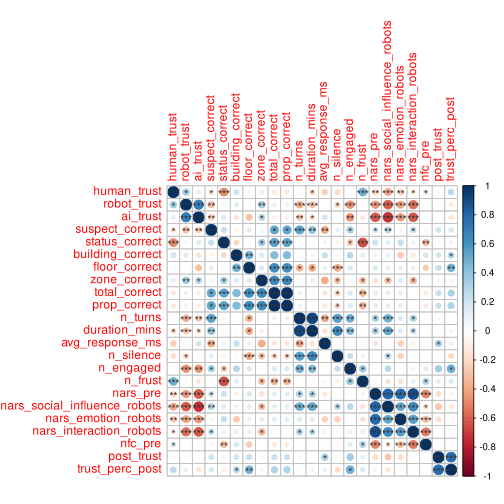
\includegraphics[keepaspectratio]{misty-paper_files/figure-pdf/unnamed-chunk-3-1.pdf}}

\pandocbounded{\includegraphics[keepaspectratio]{misty-paper_files/figure-pdf/unnamed-chunk-3-2.pdf}}

\subsection{Post-Interaction Trust
Differences}\label{post-interaction-trust-differences}

Descriptive comparisons of participant-level post-test scores indicated
an approximately 12 point difference in post-test Trust Perception
Scale-HRI scores (M ≈ 75 vs M ≈ 63) and a 27 point difference in the
Trust in Industrial Human-robot Collaboration scale (M ≈ 39 vs M ≈ 66)
between conditions, although in the first scale differences did not
reach conventional significance under a two-sample t-test (p=.10), the
second scale was significantly different between groups (p=.007).

To test these findings further, we fitted several Bayesian hierarchical
models (estimated using MCMC sampling with 4 chains of 4000 iterations
and a warmup of 1000) to predict Robot HRI-trust and Trust in HRI
Collaboration by experimental group (formula: robot\_trust\_post
\textasciitilde{} group). The model included session\_id and
trust\_items as random effects (formula: list(\textasciitilde1
\textbar{} session\_id, \textasciitilde1 \textbar{} trust\_items)). Both
models indicated higher post-interaction trust scores in the responsive
robot condition across both trust-related scales (posterior median
differences ≈ 8-15 points on a 0--100 scale).

For the Trust in Industrial Robots outcome, the responsive condition
showed a robust positive effect on post-task trust ratings. The
estimated group difference was 14.5 points (95\% CrI {[}5.62, 23.22{]}),
exceeding between-session variability and remaining stable after
accounting for item-level effects, with a 95\% chance of being large
(\textgreater6.94). In contrast, for the HRI trust perception scale, the
estimated group effect was smaller at \textasciitilde{} 9 points and
more uncertain 95\% CrI {[}-1.72, 19.25{]}, with 65\% chance of being
large (\textgreater6.87).

The posterior probability that the responsive condition increased trust
was greater than 95\% for both measures, suggesting a robust directional
effect despite substantial individual variability. Sensitivity analyses
using substantially wider priors yielded nearly identical posterior
estimates for the group effect, indicating that results were not driven
by prior specification.

In addition to directional effects, the posterior probability that the
responsive condition increased trust by at least five points was 77\% in
HRI-trust perception and 98\% in the Collaborative Trust in Industrial
Robots scale, suggesting a reasonable likelihood of a practically
meaningful effect. Moreover, in the latter collaboration scale, there is
an 85\% likelihood of an effect-size greater than 10 points.

Notably, in sessions characterized by severe communication breakdown,
the responsive robot continued to provide extended assistance and
meta-communication intended to repair the interaction. However, these
efforts did not restore mutual understanding and may have increased
participant confusion. In contrast, the control robot offered minimal,
on-demand assistance, which---while less supportive overall---may have
reduced cognitive overload under conditions of limited intelligibility.
As a result, trust ratings in breakdown sessions did not track the
intended responsiveness manipulation.

\pandocbounded{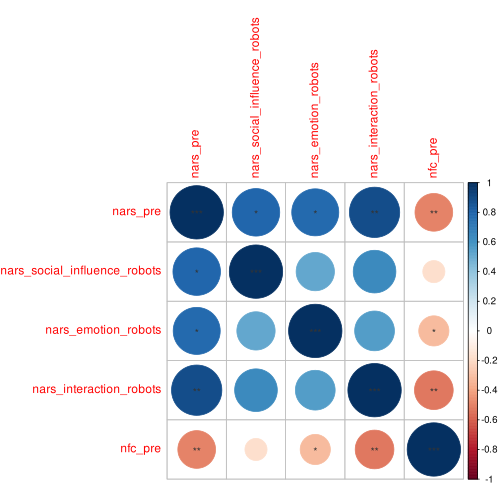
\includegraphics[keepaspectratio]{misty-paper_files/figure-pdf/unnamed-chunk-4-1.pdf}}

\pandocbounded{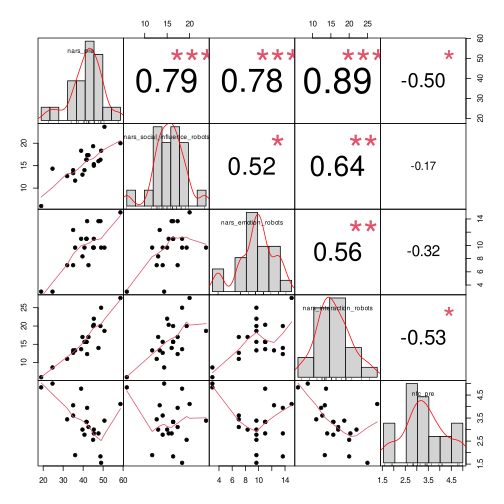
\includegraphics[keepaspectratio]{misty-paper_files/figure-pdf/unnamed-chunk-4-2.pdf}}

\subsection{Trust subscale patterns}\label{trust-subscale-patterns}

\subsection{Interaction dynamics and task
performance}\label{interaction-dynamics-and-task-performance}

\begin{table}
\fontsize{10.0pt}{12.0pt}\selectfont
\begin{tabular*}{\linewidth}{@{\extracolsep{\fill}}lcccc}
\toprule
\textbf{Characteristic} & \textbf{N} & \textbf{CONTROL}  N = 9\textsuperscript{\textit{1}} & \textbf{RESPONSIVE}  N = 14\textsuperscript{\textit{1}} & \textbf{p-value}\textsuperscript{\textit{2}} \\ 
\midrule\addlinespace[2.5pt]
post\_trust & 23 & 41 (22) & 67 (21) & {\bfseries 0.007} \\ 
post\_trust\_reliability & 23 & 41 (25) & 65 (18) & {\bfseries 0.022} \\ 
post\_trust\_perception & 23 & 39 (24) & 55 (24) & 0.14 \\ 
post\_trust\_feelings & 23 & 52 (32) & 79 (22) & {\bfseries 0.030} \\ 
Post-Task Trust Perception & 23 & 62 (15) & 77 (18) & {\bfseries 0.046} \\ 
Suspect ID Accuracy & 23 & 3 / 9 (33\%) & 9 / 14 (64\%) & 0.21 \\ 
Status Accuracy & 23 & 7 / 9 (78\%) & 9 / 14 (64\%) & 0.66 \\ 
building\_correct & 23 & 6 / 9 (67\%) & 11 / 14 (79\%) & 0.64 \\ 
floor\_correct & 23 & 6 / 9 (67\%) & 13 / 14 (93\%) & 0.26 \\ 
zone\_correct & 23 & 5 / 9 (56\%) & 4 / 14 (29\%) & 0.38 \\ 
Total Task Accuracy & 23 & 3.00 (1.12) & 3.29 (1.14) & 0.49 \\ 
Overall Task Accuracy & 23 & 0.60 (0.22) & 0.66 (0.23) & 0.49 \\ 
exclusions & 23 &  &  &  \\ 
    include &  & 9 / 9 (100\%) & 14 / 14 (100\%) &  \\ 
Dialogue Turns & 23 & 36 (7) & 33 (5) & 0.21 \\ 
Avg Task Duration (mins) & 23 & 13.82 (2.60) & 15.26 (2.12) & 0.16 \\ 
Avg Response Time (ms) & 23 & 13.21 (0.84) & 17.24 (2.52) & {\bfseries <0.001} \\ 
Silent Periods & 23 & 5.67 (2.06) & 4.71 (2.05) & 0.29 \\ 
Engaged Responses & 23 & 2.22 (2.22) & 3.50 (1.95) & 0.077 \\ 
Frustrated Responses & 23 & 0.56 (0.73) & 0.93 (1.21) & 0.58 \\ 
n\_neg & 23 & 1.00 (0.87) & 0.71 (1.07) & 0.28 \\ 
prop\_help\_requests & 23 & 0.40 (0.14) & 0.36 (0.09) & 0.48 \\ 
prop\_sentence\_frag & 23 & 0.18 (0.12) & 0.20 (0.15) & 0.92 \\ 
prop\_human\_reasoning & 23 & 0.29 (0.09) & 0.35 (0.16) & 0.37 \\ 
prop\_human\_misunderstanding & 23 & 0.02 (0.03) & 0.05 (0.09) & 0.85 \\ 
prop\_human\_affective\_engagement & 23 & 0.05 (0.05) & 0.10 (0.08) & 0.058 \\ 
prop\_robot\_helpful\_guidance & 23 & 0.68 (0.08) & 0.84 (0.08) & {\bfseries <0.001} \\ 
prop\_robot\_unhelpful & 23 & 0.08 (0.05) & 0.02 (0.03) & {\bfseries 0.004} \\ 
prop\_robot\_proactive\_checkin & 23 & 0.20 (0.08) & 0.13 (0.08) & 0.063 \\ 
prop\_robot\_encouragement & 23 & 0.00 (0.00) & 0.36 (0.11) & {\bfseries <0.001} \\ 
prop\_robot\_collaborative\_lang & 23 & 0.06 (0.04) & 0.42 (0.16) & {\bfseries <0.001} \\ 
prop\_robot\_reasoning & 23 & 0.13 (0.05) & 0.37 (0.14) & {\bfseries <0.001} \\ 
prop\_robot\_clarification & 23 & 0.22 (0.11) & 0.48 (0.14) & {\bfseries <0.001} \\ 
prop\_robot\_empathy\_expression & 23 & 0.00 (0.00) & 0.13 (0.09) & {\bfseries <0.001} \\ 
prop\_comm\_breakdown & 23 & 0.21 (0.13) & 0.22 (0.16) & >0.99 \\ 
\bottomrule
\end{tabular*}
\begin{minipage}{\linewidth}
\textsuperscript{\textit{1}}Mean (SD); n / N (\%)\\
\textsuperscript{\textit{2}}Wilcoxon rank sum test; Wilcoxon rank sum exact test; Fisher's exact test; NA\\
\end{minipage}
\end{table}

\begin{table}
\fontsize{10.0pt}{12.0pt}\selectfont
\begin{tabular*}{\linewidth}{@{\extracolsep{\fill}}lccc}
\toprule
\textbf{Characteristic} & \textbf{N} & \textbf{include}  N = 23\textsuperscript{\textit{1}} & \textbf{p-value}\textsuperscript{\textit{2}} \\ 
\midrule\addlinespace[2.5pt]
group & 23 &  &  \\ 
    CONTROL &  & 9 / 23 (39\%) &  \\ 
    RESPONSIVE &  & 14 / 23 (61\%) &  \\ 
post\_trust & 23 & 57 (24) &  \\ 
post\_trust\_reliability & 23 & 56 (24) &  \\ 
post\_trust\_perception & 23 & 49 (25) &  \\ 
post\_trust\_feelings & 23 & 68 (29) &  \\ 
Post-Task Trust Perception & 23 & 71 (18) &  \\ 
Suspect ID Accuracy & 23 & 12 / 23 (52\%) &  \\ 
Status Accuracy & 23 & 16 / 23 (70\%) &  \\ 
building\_correct & 23 & 17 / 23 (74\%) &  \\ 
floor\_correct & 23 & 19 / 23 (83\%) &  \\ 
zone\_correct & 23 & 9 / 23 (39\%) &  \\ 
Total Task Accuracy & 23 & 3.17 (1.11) &  \\ 
Overall Task Accuracy & 23 & 0.63 (0.22) &  \\ 
Dialogue Turns & 23 & 34 (6) &  \\ 
Avg Task Duration (mins) & 23 & 14.70 (2.38) &  \\ 
Avg Response Time (ms) & 23 & 15.66 (2.84) &  \\ 
Silent Periods & 23 & 5.09 (2.07) &  \\ 
Engaged Responses & 23 & 3.00 (2.11) &  \\ 
Frustrated Responses & 23 & 0.78 (1.04) &  \\ 
n\_neg & 23 & 0.83 (0.98) &  \\ 
prop\_help\_requests & 23 & 0.38 (0.11) &  \\ 
prop\_sentence\_frag & 23 & 0.19 (0.14) &  \\ 
prop\_human\_reasoning & 23 & 0.33 (0.13) &  \\ 
prop\_human\_misunderstanding & 23 & 0.04 (0.07) &  \\ 
prop\_human\_affective\_engagement & 23 & 0.08 (0.08) &  \\ 
prop\_robot\_helpful\_guidance & 23 & 0.78 (0.12) &  \\ 
prop\_robot\_unhelpful & 23 & 0.04 (0.05) &  \\ 
prop\_robot\_proactive\_checkin & 23 & 0.16 (0.08) &  \\ 
prop\_robot\_encouragement & 23 & 0.22 (0.20) &  \\ 
prop\_robot\_collaborative\_lang & 23 & 0.28 (0.22) &  \\ 
prop\_robot\_reasoning & 23 & 0.28 (0.16) &  \\ 
prop\_robot\_clarification & 23 & 0.37 (0.18) &  \\ 
prop\_robot\_empathy\_expression & 23 & 0.08 (0.09) &  \\ 
prop\_comm\_breakdown & 23 & 0.22 (0.14) &  \\ 
\bottomrule
\end{tabular*}
\begin{minipage}{\linewidth}
\textsuperscript{\textit{1}}n / N (\%); Mean (SD)\\
\textsuperscript{\textit{2}}NA\\
\end{minipage}
\end{table}

\subsubsection{Task performance}\label{task-performance}

Objective task accuracy did not differ between conditions across any
task-level measures except suspect accuracy (robot dependendant task),
indicating that increased trust was only attributable to improved task
success when interaction was necessary to complete accurately.

Despite similar task accuracy, interactions in the responsive condition
were characterized by longer durations, slower response times, and a
higher number of AI-detected engaged responses. These findings suggest
that responsiveness altered the interaction dynamics and affective tone
rather than task outcomes.

\subsection{Individual differences and correlational
patterns}\label{individual-differences-and-correlational-patterns}

As expected, we found that higher Need for Cognition (NFC) scores were
negatively associated with Negative Attitudes Towards Robots (NARS),
indicating that individuals who enjoy effortful thinking tend to have
more positive attitudes towards robots. This relationship is consistent
with prior literature suggesting that cognitive engagement is associated
with openness to new technologies. In terms of NARS subscales, NFC was
negatively correlated with all three subscales, but significantly so
only in the domain of Situations of Interaction with Robots. This
suggests that individuals with higher NFC are less likely to hold
negative attitudes across various dimensions of robot interaction but
especially around direct interaction with robots.

--\textgreater{} how to talk about post-interaction correlations
w/pre-interaction measures Several behavioural and task-level measures
were correlated with post-interaction trust, consistent with the
interpretation that trust judgments were shaped by interaction quality;
these variables were not included as covariates in primary models to
avoid conditioning on potential mediators.

Baseline negative attitudes toward robots were negatively correlated
with post-interaction trust, with the strongest associations observed
for affective trust subscales. In contrast, objective task performance
was selectively associated with perceived reliability. Need for
cognition was negatively correlated with negative robot attitudes and
interaction-level negative affect, suggesting that individual
differences contributed to variability in trust responses.

\begin{figure}

\centering{

\pandocbounded{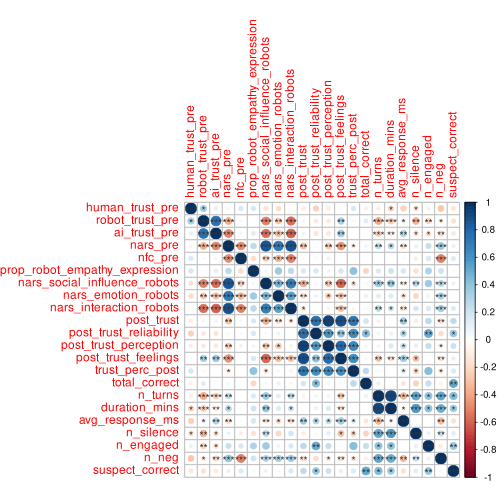
\includegraphics[keepaspectratio]{misty-paper_files/figure-pdf/fig-corr-1.pdf}}

}

\caption{\label{fig-corr}}

\end{figure}%

\subsubsection{Model robustness and predictive
checks}\label{model-robustness-and-predictive-checks}

Sensitivity analyses using alternative prior specifications yielded
substantively similar estimates, and leave-one-out cross-validation
indicated comparable predictive performance between models with and
without the group effect.

\begin{tcolorbox}[enhanced jigsaw, left=2mm, opacitybacktitle=0.6, colframe=quarto-callout-important-color-frame, arc=.35mm, toptitle=1mm, opacityback=0, titlerule=0mm, bottomrule=.15mm, rightrule=.15mm, coltitle=black, bottomtitle=1mm, colbacktitle=quarto-callout-important-color!10!white, title=\textcolor{quarto-callout-important-color}{\faExclamation}\hspace{0.5em}{TO DO:}, toprule=.15mm, breakable, colback=white, leftrule=.75mm]

\begin{itemize}
\tightlist
\item
  add subscale column to long format data
\item
  run an analysis of performance by robot-dependent versus
  robot-independent tasks
\item
  write up a future directions section for the planned larger study
\item
  talk about unexpected language issues with people signing up with
  difficultly speaking and understanding english which cuased problems
  with asr and interaction
\item
  run analysis of dialogue dynamics included Bertopic or some other
  analysis of the actual content of the conversations/interactions
\end{itemize}

\end{tcolorbox}

\begin{tcolorbox}[enhanced jigsaw, left=2mm, opacitybacktitle=0.6, colframe=quarto-callout-important-color-frame, arc=.35mm, toptitle=1mm, opacityback=0, titlerule=0mm, bottomrule=.15mm, rightrule=.15mm, coltitle=black, bottomtitle=1mm, colbacktitle=quarto-callout-important-color!10!white, title=\textcolor{quarto-callout-important-color}{\faExclamation}\hspace{0.5em}{TODO2}, toprule=.15mm, breakable, colback=white, leftrule=.75mm]

Manually score each dialogue series.

For each interaction and stage:

\begin{itemize}
\tightlist
\item
  did the participant ask for help?
\item
  how many times?
\item
  did the robot give useful help?
\item
  did the robot give misleading or incorrect help?
\item
  did the robot stick to the policy?
\item
  how many times did the robot fail to understand the participant?
\end{itemize}

For each task:

\begin{itemize}
\tightlist
\item
  is there evidence that the robot helped complete the task?
\item
  is there evidence that the participant solved the problem without
  help?
\end{itemize}

\end{tcolorbox}

Need to discuss that these items were on a 0-100 scale that required
sliding a bar, while the other trust scale was on a 1-5 Likert that
required simply clicking. The post test was administered on a laptop
with a trackpad which may have caused difficulties for some participants
who found it difficult to drag the slider with the trackpad. This could
have introduced additional noise into the measurement of this scale,
which may explain why the effects were somewhat weaker here.

\section{Discussion}\label{discussion}

Mention language confounders!!

The second task was intentionally designed to be sufficiently
challenging that completing it within the allotted time was difficult
without assistance. This ensured that interaction with the robot
represented a meaningful opportunity for collaboration rather than a
trivial or purely optional exchange. By contrasting a robot-dependent
task with an open-ended advisory task, the study examined trust
formation across interaction contexts that varied in both informational
asymmetry and reliance on the robot.

This pilot study examined trust outcomes following in-person interaction
with an autonomous social robot under two interaction policies: a
responsive, affect-adaptive condition and a neutral, non-responsive
control condition. By leveraging a fully autonomous dialogue system
integrated with speech recognition and affect detection, the study aimed
to evaluate how robot responsiveness influences trust formation in
realistic human--robot collaboration scenarios.

Descriptive comparisons of post-interaction measures indicated that
participants in the responsive condition reported consistently higher
trust across all trust measures, with differences ranging from
approximately 8 to 16 points on a 0--100 scale, although uncertainty
remained high given the small sample. Notably, the responsive condition
did not differ from control in objective task accuracy, suggesting that
increased trust was not driven by improved task success. Instead,
responsive interactions were characterized by longer durations, slower
response times, and a higher number of AI-detected engaged responses,
indicating a shift in interaction dynamics rather than performance.

Baseline negative attitudes toward robots were most strongly associated
with affective components of trust rather than perceptions of
reliability, suggesting that pre-existing attitudes primarily shape
emotional responses to interaction rather than judgments of system
competence. Conversely, objective task performance was selectively
associated with perceived reliability, indicating that participants
distinguished between affective and functional aspects of trust.

Future work with larger samples could formally test mediation pathways
linking robot responsiveness, interaction fluency, affective responses,
and trust judgments, as well as moderation by baseline attitudes toward
robots and need for cognition.

Participants in the responsive condition also exhibited higher levels of
AI-detected engagement during interaction, as indexed by a greater
number of responses classified as positive affect (t-test result). This
suggests that responsive behaviours altered the affective tone of the
interaction itself.

\subsection{Technical challenges}\label{technical-challenges}

\begin{itemize}
\tightlist
\item
  Need to talk about language issues with participants who had
  difficulty speaking and understanding English which caused problems
  with ASR and interaction.
\item
  Need to talk about issues where the AI was not able to flexibly handle
  when people asked a question about the suspect that was close to or
  another word for a ground-truth feature but not exactly the same word,
  causing confusion and miscommunication. E.g., ``Was the suspect
  wearing pink?'' The ground-truth feature was top: PINK, top-type:
  HOODIE; but the ASR and NLU did not extrapolate to understand that
  ``wearing pink'' referred to the same feature as ``top: PINK'',
  causing confusion and miscommunication. Maybe the prompt could have
  included some examples of different phrasing which could improve this?
  To solve this issue in future work, we can expand the NLU training
  data to include more paraphrases and synonyms for each feature.
\end{itemize}

There was also a case where someone asked `is the top shirt hoodie red?'
to which the AI answered YES. It may have been confused by the multiple
descriptors in the question. Future work could involve improving the NLU
to handle more complex queries with multiple attributes.

Discuss future work where we will look investigate the `embodied' effect
of having a physical robot versus a virtual agent on trust and
collaboration in HRI.

Also, prompt could include examples of what to do when dialogue appears
fragmented, to remind participants to wait until the blue light is on
before speaking and to switch up its phrasing if the robot seems to not
understand.

Also, the control condition seemed to be somewhat neutered in terms of
flexibility in responding in different ways. it would always respond
with the exact same phrase when confronted with a sentence fragment or a
question it could not directly answer.

Also issues with people not paying attention to the robot's visual cues
to know when to speak, leading to more fragmented dialogue. Future work
could involve improving participant instructions, improved latency and
`listening' \ldots{} and the robot's feedback mechanisms to better
manage turn-taking.

Need to remember to flag participants who did not complete/skipped
specific tasks. E.g. P56 skipped the wrapup entirely. Many skipped the
brief (by advancing on their own through the dashboard).

\section{Conclusion and Future Work}\label{conclusion-and-future-work}

\section{Appendix}\label{appendix}

\subsection{Dialogue Coding Scheme}\label{dialogue-coding-scheme}

\subsubsection{Task Outcome Layer
(Stage-Level)}\label{task-outcome-layer-stage-level}

\begin{longtable}[]{@{}
  >{\raggedright\arraybackslash}p{(\linewidth - 4\tabcolsep) * \real{0.3333}}
  >{\raggedright\arraybackslash}p{(\linewidth - 4\tabcolsep) * \real{0.3333}}
  >{\raggedright\arraybackslash}p{(\linewidth - 4\tabcolsep) * \real{0.3333}}@{}}
\toprule\noalign{}
\begin{minipage}[b]{\linewidth}\raggedright
Variable
\end{minipage} & \begin{minipage}[b]{\linewidth}\raggedright
Type
\end{minipage} & \begin{minipage}[b]{\linewidth}\raggedright
Description
\end{minipage} \\
\midrule\noalign{}
\endhead
\bottomrule\noalign{}
\endlastfoot
\texttt{task\_outcome} & categorical & Final task status
(\texttt{completed}, \texttt{timeout}, \texttt{skipped},
\texttt{partial}, \texttt{abandoned}). Exactly one per task. \\
\texttt{task\_completed} & binary & Task goal was fully completed within
the allotted time. \\
\texttt{task\_timed\_out} & binary & Task ended due to expiration of the
time limit before completion. \\
\texttt{task\_skipped} & binary & Participant explicitly skipped or
advanced past the task without completing it. \\
\texttt{task\_partially\_completed} & binary & Task progress was made,
but the full solution was not reached. \\
\texttt{task\_abandoned} & binary & Participant disengaged or stopped
attempting the task before timeout. \\
\texttt{task\_time\_remaining\_sec} & numeric & Time remaining (in
seconds) when the task ended; 0 if timed out. \\
\texttt{task\_completed\_without\_help} & binary & Task was completed
without any help requests to the robot. \\
\texttt{task\_required\_robot\_help} & binary & At least one robot help
interaction was required for task completion. \\
\end{longtable}

\subsubsection{Dialogue Interaction Layer
(Turn-Level)}\label{dialogue-interaction-layer-turn-level}

\paragraph{Human Turn Codes}\label{human-turn-codes}

\begin{longtable}[]{@{}
  >{\raggedright\arraybackslash}p{(\linewidth - 4\tabcolsep) * \real{0.3333}}
  >{\raggedright\arraybackslash}p{(\linewidth - 4\tabcolsep) * \real{0.3333}}
  >{\raggedright\arraybackslash}p{(\linewidth - 4\tabcolsep) * \real{0.3333}}@{}}
\toprule\noalign{}
\begin{minipage}[b]{\linewidth}\raggedright
Variable
\end{minipage} & \begin{minipage}[b]{\linewidth}\raggedright
Type
\end{minipage} & \begin{minipage}[b]{\linewidth}\raggedright
Description
\end{minipage} \\
\midrule\noalign{}
\endhead
\bottomrule\noalign{}
\endlastfoot
\texttt{human\_help\_request} & binary & Participant explicitly or
implicitly asks the robot for help or guidance. \\
\texttt{human\_reasoning\_self} & binary & Participant articulates their
own reasoning or problem-solving independent of the robot. \\
\texttt{human\_confusion} & binary & Participant expresses confusion or
uncertainty. \\
\texttt{human\_confirmation\_seeking} & binary & Participant seeks
confirmation of a tentative belief or solution. \\
\texttt{human\_ignores\_robot} & binary & Participant proceeds without
engaging with the robot's prior input. \\
\end{longtable}

\paragraph{Robot Turn Codes}\label{robot-turn-codes}

\begin{longtable}[]{@{}
  >{\raggedright\arraybackslash}p{(\linewidth - 4\tabcolsep) * \real{0.3333}}
  >{\raggedright\arraybackslash}p{(\linewidth - 4\tabcolsep) * \real{0.3333}}
  >{\raggedright\arraybackslash}p{(\linewidth - 4\tabcolsep) * \real{0.3333}}@{}}
\toprule\noalign{}
\begin{minipage}[b]{\linewidth}\raggedright
Variable
\end{minipage} & \begin{minipage}[b]{\linewidth}\raggedright
Type
\end{minipage} & \begin{minipage}[b]{\linewidth}\raggedright
Description
\end{minipage} \\
\midrule\noalign{}
\endhead
\bottomrule\noalign{}
\endlastfoot
\texttt{robot\_helpful\_guidance} & binary & Robot provides accurate,
task-relevant guidance. \\
\texttt{robot\_misleading\_guidance} & binary & Robot provides
misleading or incorrect guidance. \\
\texttt{robot\_factually\_incorrect} & binary & Robot states information
that is objectively incorrect. \\
\texttt{robot\_policy\_violation} & binary & Robot violates stated
system or task constraints. \\
\texttt{robot\_on\_policy\_unhelpful} & binary & Robot adheres to policy
but provides vague or non-actionable assistance. \\
\texttt{robot\_stt\_failure} & binary & Robot response reflects a
speech-to-text or input understanding failure. \\
\texttt{robot\_clarification\_request} & binary & Robot asks the
participant to repeat or clarify their input. \\
\end{longtable}

\subsubsection{Affective Interaction Layer
(Turn-Level)}\label{affective-interaction-layer-turn-level}

\paragraph{Robot Affective Behavior}\label{robot-affective-behavior}

\begin{longtable}[]{@{}
  >{\raggedright\arraybackslash}p{(\linewidth - 4\tabcolsep) * \real{0.3333}}
  >{\raggedright\arraybackslash}p{(\linewidth - 4\tabcolsep) * \real{0.3333}}
  >{\raggedright\arraybackslash}p{(\linewidth - 4\tabcolsep) * \real{0.3333}}@{}}
\toprule\noalign{}
\begin{minipage}[b]{\linewidth}\raggedright
Variable
\end{minipage} & \begin{minipage}[b]{\linewidth}\raggedright
Type
\end{minipage} & \begin{minipage}[b]{\linewidth}\raggedright
Description
\end{minipage} \\
\midrule\noalign{}
\endhead
\bottomrule\noalign{}
\endlastfoot
\texttt{robot\_empathy\_expression} & binary & Robot expresses empathy,
encouragement, or reassurance. \\
\texttt{robot\_emotion\_acknowledgement} & binary & Robot explicitly
references an inferred participant emotional state. \\
\texttt{robot\_affect\_task\_aligned} & binary & Robot's affective
response is appropriate and supportive in context. \\
\texttt{robot\_affect\_misaligned} & binary & Robot's affective response
is mistimed or disruptive to the task. \\
\end{longtable}

\paragraph{Human Affective Response}\label{human-affective-response}

\begin{longtable}[]{@{}
  >{\raggedright\arraybackslash}p{(\linewidth - 4\tabcolsep) * \real{0.3333}}
  >{\raggedright\arraybackslash}p{(\linewidth - 4\tabcolsep) * \real{0.3333}}
  >{\raggedright\arraybackslash}p{(\linewidth - 4\tabcolsep) * \real{0.3333}}@{}}
\toprule\noalign{}
\begin{minipage}[b]{\linewidth}\raggedright
Variable
\end{minipage} & \begin{minipage}[b]{\linewidth}\raggedright
Type
\end{minipage} & \begin{minipage}[b]{\linewidth}\raggedright
Description
\end{minipage} \\
\midrule\noalign{}
\endhead
\bottomrule\noalign{}
\endlastfoot
\texttt{human\_affective\_engagement} & binary & Participant responds in
a socially warm or emotionally engaged manner. \\
\texttt{human\_social\_reciprocity} & binary & Participant mirrors or
responds to the robot's affective expression. \\
\texttt{human\_anthropomorphic\_language} & binary & Participant treats
the robot as a social agent. \\
\texttt{human\_emotional\_disengagement} & binary & Participant responds
in a curt, dismissive, or withdrawn manner. \\
\end{longtable}

\subsubsection{Notes}\label{notes}

\begin{itemize}
\tightlist
\item
  Turn-level variables are coded per dialogue turn.
\item
  Task outcome variables are coded once per
  \texttt{session\_id\ ×\ stage}.
\item
  Raw dialogue text was retained during coding and removed prior to
  aggregation.
\item
  Multiple turn-level codes may co-occur unless otherwise specified.
\end{itemize}

\subsection{Key Components of the
System}\label{key-components-of-the-system}

This study implemented a multi-stage collaborative task system where
participants collaborate with the Misty II social robot to solve a
who-dunnit type task. The system utilizes an autonomous,
mixed-initiative dialogue architecture via langchain with
affect-responsive capabilities.

\begin{enumerate}
\def\labelenumi{\arabic{enumi}.}
\item
  Misty-II Robot: A programmable robot platform equipped with sensors
  and actuators for interaction.
\item
  Automated Speech Recognition (ASR): A speech-to-speech pipeline that
  processes spoken input from users and converts it into text for LLM
  processing then back to speech for output on the robot.

  \begin{itemize}
  \tightlist
  \item
    STT: Deepgram API for real-time speech-to-text conversion.
  \item
    DistilRoBERTa-base fine-tuned on emotion classification for emotion
    detection from user utterances
  \item
    LLM: Gemini API for processing text input and generating
    contextually relevant responses in JSON format
  \item
    TTS: Misty-II text-to-speech (TTS) engine on 820 processor.
  \end{itemize}
\item
  Langchain Dialogue Management: A system that manages the flow of
  conversation, ensuring coherent and contextually appropriate dialogue
  within a two-part collaborative task.
\item
  Collaborative-Tasks

  \begin{itemize}
  \tightlist
  \item
    Task 1: Whodunnit style task where human and robot collaborate to
    find a missing robot via the human asking Yes/No questions (process
    of elimination in 6x4 suspect grid) to the robot. Robot knows ground
    truth but can only answer Yes/No questions about suspect features.
    Can not directly describe the suspect or name them. (human can
    choose a random suspect to solve on their own but only 1 in 24
    chance of being correct without robot help)
  \item
    Task 2: Where is Atlas? Robot collaborates with human to find Atlas
    by deciphering cryptic system and sensor logs. Robot does not know
    the answer here and can only guide the human usinng its expertise
    and knowledge of computer systems and basic logical reasoning.
    (human can solve on their own but very difficult without robot help
    depending on participants technical background).
  \end{itemize}
\item
  Flask-gui dashboard interface: A web-based interface/dashboard that
  allowed participants to interact with the tasks, view task-related
  information and input their answers to the questions. Responses were
  sent to the robot to signal task progression.

  \begin{itemize}
  \tightlist
  \item
    Task 1 dashboard: Displays the suspect grid and allows the user to
    select suspects and view their features.
  \item
    Task 2 dashboard: Displays system logs and allows the user to input
    their findings.
  \end{itemize}
\item
  Pre and post tests:

  \begin{itemize}
  \tightlist
  \item
    PRE-TESTS: Need for Cognition Scale (short); Negative Attitudes to
    Robots Scale (NARS);
  \item
    POST-TESTS: Trust Perception Scale-HRI; 9 custom questions adapted
    from Charalambous et al.~(2020) on trust in industrial human-robot
    collaboration;
  \end{itemize}
\end{enumerate}

\section{Technical Specifications}\label{technical-specifications}

\subsection{System Overview}\label{system-overview}

This study implements a multi-stage collaborative task system where
participants collaborate with the Misty II social robot to solve a
who-dunniti type task. The system utilizes an autonomous,
mixed-initiative dialogue architecture with affect-responsive
capabilities.

\subsection{Hardware Platform}\label{hardware-platform}

\textbf{Robot}: Misty II Social Robot (Furhat Robotics)

\begin{itemize}
\tightlist
\item
  Mobile social robot platform with expressive display, arm actuators,
  and head movement
\item
  RGB LED for state indication
\item
  RTSP video streaming (1920×1080, 30fps) for audio capture
\item
  Custom action scripting for synchronized multimodal expressions
\end{itemize}

\subsection{Software Architecture}\label{software-architecture}

\subsubsection{Core System Components}\label{core-system-components}

\textbf{Programming Language}: Python 3.10

\textbf{Primary Dependencies}:

\begin{itemize}
\tightlist
\item
  \texttt{misty-sdk} (Python SDK for Misty Robotics API) - Robot control
  and sensor access
\item
  \texttt{deepgram-sdk} (4.8.1) - Speech-to-text processing
\item
  \texttt{ffmpeg-python} (0.2.0) - Audio stream processing
\item
  \texttt{flask} (3.1.2) + \texttt{flask-socketio} (5.5.1) - Web
  interface for task presentation
\item
  \texttt{duckdb} (1.4.0) - Experimental data logging database
\end{itemize}

\subsubsection{Large Language Models}\label{large-language-models}

\textbf{LLM Provider}:

\textbf{Google Gemini}:

\begin{itemize}
\tightlist
\item
  Model: \texttt{gemini-2.5-flash-lite} (configurable via environment
  variable)
\item
  Integration: \texttt{langchain-google-genai} with
  \texttt{google-generativeai} API
\item
  Response format: JSON-only output
  (\texttt{response\_mime\_type:\ "application/json"}). This format is
  required by Misty-II for reliable parsing and for action execution.
\end{itemize}

\textbf{LLM Configuration}:

\begin{itemize}
\tightlist
\item
  Temperature: 0.7 (for balanced creativity and coherence)
\item
  Memory: Conversation buffer memory with file-based persistence
  (\texttt{langchain.memory.ConversationBufferMemory})
\item
  Context window: Full conversation history maintained across
  interaction stages but reset between sessions.
\end{itemize}

\subsection{LangChain Framework
Integration}\label{langchain-framework-integration}

\subsubsection{Core LangChain
Components}\label{core-langchain-components}

\textbf{Framework Version}: \texttt{langchain-core} with modular
provider packages

\begin{itemize}
\tightlist
\item
  \texttt{langchain} (meta-package)
\item
  \texttt{langchain-community} (0.3.31)
\item
  \texttt{langchain-google-genai} Gemini integration
\end{itemize}

\subsubsection{ConversationChain
Architecture}\label{conversationchain-architecture}

\textbf{Memory Management} (\texttt{ConversationChain} class in
\texttt{conversation\_chain.py}):

\begin{enumerate}
\def\labelenumi{\arabic{enumi}.}
\tightlist
\item
  \textbf{Conversation Buffer Memory}:

  \begin{itemize}
  \tightlist
  \item
    Implementation: \texttt{langchain.memory.ConversationBufferMemory}
  \item
    Storage: File-based persistent chat history
    (\texttt{FileChatMessageHistory})
  \item
    Format: JSON files in \texttt{.memory/} directory, one per
    participant session
  \item
    Memory key: \texttt{"history"}
  \item
    Return format: Message objects (full conversation context)
  \end{itemize}
\item
  \textbf{Memory Reset Policy}:

  \begin{itemize}
  \tightlist
  \item
    Default: Reset on each new session launch
  \item
    Archive previous session: Timestamped archive files stored in
    \texttt{.memory/archive/}
  \item
    Configuration: \texttt{RESET\_MEMORY} and \texttt{ARCHIVE\_MEMORY}
    environment variables
  \end{itemize}
\end{enumerate}

\subsubsection{Prompt Construction}\label{prompt-construction}

\textbf{Message Structure}

(LangChain message types):
\texttt{python\ {[}SystemMessage,\ *history\_messages,\ HumanMessage{]}}

System Message Assembly:

\begin{itemize}
\tightlist
\item
  Core instructions (task framing, role definition)
\item
  Personality instructions (mode-specific behaviour)
\item
  Stage-specific instructions (current task context)
\item
  Output format constraints (JSON schema specification)
\end{itemize}

\begin{verbatim}
Human Message Format:   {     
"user": "<transcribed_speech>",     
"stage": "<current_stage>",     
"detected_emotion": "<emotion_label>",     
"frustration_note": "<optional_alert>",     
"timer_expired": "<task_id>",     ...   }
\end{verbatim}

\begin{itemize}
\tightlist
\item
  JSON-encoded context variables passed alongside user input
\item
  Enables LLM to access environmental state without breaking message
  history
\end{itemize}

\subsubsection{Memory Persistence:}\label{memory-persistence}

\begin{itemize}
\tightlist
\item
  Save after each turn: memory.save\_context(\{``input'': user\_text\},
  \{``output'': llm\_response\})
\item
  Maintains conversational coherence across multi-stage interaction
\item
  Enables LLM to reference previous exchanges (e.g., ``As I mentioned
  earlier\ldots{}'')
\end{itemize}

\subsubsection{LangChain Design
Rationale}\label{langchain-design-rationale}

Why LangChain for this application:

\begin{enumerate}
\def\labelenumi{\arabic{enumi}.}
\tightlist
\item
  Memory abstraction: Automatic conversation history management without
  manual message list handling
\item
  Provider flexibility: Easy switching between Gemini and OpenAI without
  rewriting prompt logic
\item
  Message typing: Structured SystemMessage/HumanMessage/AIMessage types
  maintain role clarity
\item
  File persistence: Built-in FileChatMessageHistory enables session
  recovery and archiving
\item
  Future extensibility: Framework supports adding tools, retrieval, or
  multi-agent patterns if needed
\end{enumerate}

Alternatives considered: Direct API calls would reduce dependencies but
require reimplementing conversation history management, prompt
templating, and cross-provider compatibility layers.

\subsubsection{LangChain Limitations in This
Context}\label{langchain-limitations-in-this-context}

\begin{itemize}
\tightlist
\item
  No chains used: Despite name ConversationChain, this is a direct LLM
  wrapper (no LangChain Expression Language chains)
\item
  No tools/agents: Simple request-response pattern (could extend for
  future tool-use capabilities)
\item
  Custom JSON parsing: LangChain's built-in output parsers not used;
  custom extraction handles malformed responses more robustly
\end{itemize}

\subsubsection{Speech Processing}\label{speech-processing}

\textbf{Speech-to-Text (STT)}:

\begin{itemize}
\tightlist
\item
  Provider: Deepgram Nova-2 (\texttt{deepgram-sdk} 4.8.1)
\item
  Model: \texttt{nova-2} with US English (\texttt{en-US})
\item
  Smart formatting enabled
\item
  Interim results for real-time partial transcription
\item
  Voice Activity Detection (VAD) events
\item
  Adaptive endpointing: 200ms (conversational stages) / 500ms
  (log-reading task)
\item
  Utterance end timeout: 1000ms (conversational) / 2000ms (log-reading)
\item
  Audio processing: RTSP stream from Misty → FFmpeg MP3 encoding →
  Deepgram WebSocket
\end{itemize}

\textbf{Text-to-Speech (TTS)} - Three options:

\begin{enumerate}
\def\labelenumi{\arabic{enumi}.}
\item
  \textbf{Misty Onboard TTS} (this is the one we used): Native robot
  voice via onboard TTS
\item
  \textbf{OpenAI TTS}:

  \begin{itemize}
  \tightlist
  \item
    Model: \texttt{tts-1} (low-latency variant)
  \item
    Voice: \texttt{sage}
  \item
    Format: MP3, served via HTTP (port 8000)
  \item
    Ultimately chose not to use because we wanted a more robotic,
    non-human voice
  \item
    Didn't want the human voice influencing trust on its own (future
    research could look at trust in relation to type of voice)
  \end{itemize}
\item
  \textbf{Deepgram Aura}:

  \begin{itemize}
  \tightlist
  \item
    Model: \texttt{aura-stella-en} (conversational female voice)
  \item
    Format: MP3, served via HTTP
  \item
    Ultimately chose not to use because we wanted a more robotic,
    non-human voice
  \end{itemize}
\end{enumerate}

\subsubsection{Emotion Detection}\label{emotion-detection}

\textbf{Model}: DistilRoBERTa-base fine-tuned on emotion classification

\begin{itemize}
\tightlist
\item
  HuggingFace identifier:
  \texttt{j-hartmann/emotion-english-distilroberta-base}
\item
  Framework: \texttt{transformers} (4.57.1) pipeline
\item
  Hardware: CUDA GPU acceleration (automatic fallback to CPU)
\item
  Output classes: joy, anger, sadness, fear, disgust, surprise, neutral
\item
  Mapped to interaction states: positively engaged, irritated,
  disappointed, anxious, frustrated, curious, neutral
\end{itemize}

\subsubsection{Multimodal Robot
behaviour}\label{multimodal-robot-behaviour}

\textbf{Expression System}: 25 custom action scripts combining:

\begin{itemize}
\tightlist
\item
  LLM was prompted to choose an appropriate expression from a predefined
  set based on context.
\item
  Facial displays (image eye-expression files on screen)
\item
  LED color patterns (solid, breathe, blink)
\item
  Arm movements (bilateral position control)
\item
  Head movements (pitch, yaw, roll control)
\end{itemize}

\textbf{Nonverbal Backchannel behaviours} (RESPONSIVE mode only):

\begin{itemize}
\tightlist
\item
  Real-time listening cues triggered by partial transcripts
  (disfluencies, hesitation markers)
\item
  Emotion-matched expressions (e.g., ``concern'' for hesitation,
  ``excited'' for breakthroughs)
\end{itemize}

\textbf{LED State Indicators}:

\begin{itemize}
\tightlist
\item
  Blue (0, 199, 252): Actively listening (microphone open)
\item
  Purple (100, 70, 160): Processing/speaking (microphone closed)
\end{itemize}

\subsection{Data Collection}\label{data-collection}

\textbf{Database}: DuckDB relational database
(\texttt{experiment\_data.duckdb})

\textbf{Logged Data}:

1. \textbf{Sessions table}: participant ID (auto-incremented P01,
P02\ldots), condition assignment, timestamps, duration

2. \textbf{Dialogue turns table}: turn-by-turn user input, LLM response,
expression, response latency (ms), behavioural flags

3. \textbf{Task responses table}: submitted answers with timestamps and
time-on-task

4. \textbf{Events table}: stage transitions, silence check-ins, timer
expirations, detected emotions

\subsection{Interaction Dynamics}\label{interaction-dynamics}

\subsubsection{Silence Handling}\label{silence-handling}

\textbf{Silence detection}: 25-second threshold triggers check-in prompt

\begin{itemize}
\tightlist
\item
  RESPONSIVE: ``Still working on it? No rush - I'm here if you need
  help!''
\item
  CONTROL: ``I am ready when you have a question.''
\end{itemize}

\subsubsection{Emotion-Responsive behaviours (RESPONSIVE condition
only)}\label{emotion-responsive-behaviours-responsive-condition-only}

\textbf{Frustration tracking}:

\begin{itemize}
\tightlist
\item
  Consecutive detection of frustrated/anxious/irritated/disappointed
  states
\item
  Threshold: ≥2 consecutive frustrated turns triggers proactive support
\item
  RESPONSIVE adaptation: ``This part can be tough. Want me to walk you
  through it?''
\end{itemize}

\textbf{Positive emotion matching}:

\begin{itemize}
\tightlist
\item
  Celebratory language for curious/engaged states
\item
  Momentum maintenance: ``Yes! Great observation!''
\end{itemize}

\textbf{Run Mode}: Set programmatically in \texttt{mistyGPT\_emotion.py}
line 126:

\begin{Shaded}
\begin{Highlighting}[]
\NormalTok{RUN\_MODE }\OperatorTok{=} \StringTok{"RESPONSIVE"}  \CommentTok{\# or "CONTROL"}
\end{Highlighting}
\end{Shaded}

\subsection{Prompt Engineering}\label{prompt-engineering}

Modular prompt system (PromptLoader class):

\begin{itemize}
\tightlist
\item
  core\_system.md: Task framing, role description, output format schema
\item
  role\_responsive.md / role\_control.md: Condition-specific personality
  instructions
\item
  stage1\_greeting.md through stage5\_wrap\_up.md: Stage-specific task
  instructions.
\end{itemize}

Context injection: Real-time contextual variables passed to LLM:

\begin{itemize}
\tightlist
\item
  Current stage
\item
  Detected emotion (if enabled)
\item
  Task submission status
\item
  Timer expiration notifications
\item
  Silence check-in flags
\end{itemize}

\subsection{Inter-process
Communication}\label{inter-process-communication}

Flask REST API endpoints:

\begin{itemize}
\tightlist
\item
  GET /stage\_current: Synchronize stage state with facilitator GUI
\item
  GET /task\_submission\_status: Detect participant task submissions
\item
  GET /timer\_expired\_status: Detect timer expirations
\item
  POST /stage: Update stage (facilitator override)
\item
  POST /reset\_timer: Clear timer expiration flags
\end{itemize}


\bibliography{bibliography.bib}



\end{document}
